\documentclass[10pt]{paper}
\usepackage{amsmath}
\usepackage{graphicx}
\usepackage{xcolor}
\usepackage{booktabs}
\usepackage[hyphens]{url}

\newcommand{\po}{\mathsf{po}}
\newcommand{\poloc}{\mathsf{po\text{-}loc}}
\newcommand{\co}{\mathsf{co}}
\newcommand{\rf}{\mathsf{rf}}
\newcommand{\fr}{\mathsf{fr}}
\newcommand{\com}{\mathsf{com}}
\newcommand{\loc}{\mathsf{loc}}
\newcommand{\axiom}[1]{\textsc{#1}}
\newcommand{\litmus}[1]{\texttt{#1}}
\newcommand{\state}[1]{\texttt{#1}}

\newcommand{\match}{\;\mathsf{match}\;}

\newcommand{\JAComment}[1]{\textcolor{red}{(Jade: #1)}}
\newcommand{\NCComment}[1]{\textcolor{green}{(Nathan: #1)}}
\newcommand{\DSComment}[1]{\textcolor{blue}{(Daryl: #1)}}

\begin{document}
\title{Linking Architecture and Microarchitecture with Cats and Dogs}
\author{Jade Alglave\and Nathan Chong\and Daryl Stewart}
\maketitle

\begin{abstract}
We report on work to address the problem of formally linking a specification to an implementation in hardware design.
%
More specifically, the memory consistency model (architecture) with respect to the design of a L1 memory system (microarchitecture).
\end{abstract}

Determining if a design meets or is within the envelope of a specification is a key problem in design integrity.
%
This is a particularly difficult problem if the specification is large or subtle, as in the case of the ARM architecture (which is both).
%
Common and valuable approaches to this problem are code reviews, testing and block-level assertions.
%
In this report, we look at linking the work of Alglave et al.~\cite{cats}, for reasoning about memory models (i.e., architecture), with the work of Stewart et al.~\cite{dogs}, for defining and checking end-to-end properties of a processor memory system (i.e., microarchitecture).

\section{Background}

\subsection{Cats}

Cats is a generic framework for defining and exploring (axiomatic\footnote{Operational semantics is an alternative approach}) formalisations of memory models.
%
In this work a memory model is a set of axioms, expressed as relations and orders over the set of memory events, that can be `run', using the herd tool, over a given litmus test to automatically explore possible execution behaviours.

A litmus test is a multiprocessor program giving a sequence of instructions (e.g., \texttt{LDR} and \texttt{STR}) per thread.
%
A litmus test gives rise to a set of behaviours or \emph{candidate executions} (containing events such as reads and writes) that can be checked with respect to the memory model axioms.
%
If any axiom is violated then the execution is forbidden (i.e, an implementation must never exhibit this behaviour); otherwise, the execution is allowed by the architecture (i.e., an implementation may exhibit this behaviour).

For example, the ARM model in herd defines the axiom
  \axiom{SC-PER-LOC} (sequential consistency per location)
as
  $\texttt{acyclic} (\poloc \cup \com)$,
where
  $\poloc = \po \cap \loc$
and
  $\com = \co \cup \rf \cup \fr$.

The relation $\po$ (program order) is defined between events arising from instructions executing on the same thread;
%
$\co$ (coherence order) is a total order over writes to the same location;
%
$\rf$ (reads-from) is a relation that connects a write to a read of the same location (where the value read is the same as the value written);
%
and, finally, the $\fr$ (from-reads) relation is induced by $\co$ and $\rf$: if a write $w$ is $\co$-before a write $w'$ and $r$ reads-from $w$ then $r$ from-reads $w'$.

Now, consider the following litmus test, known as \litmus{coRR}:
%
\begin{verbatim}
  // [x] = 0 initially
  // P0         |   P1
  STR [x], #1   |   LDR r0, [x]
                |   LDR r1, [x]
\end{verbatim}

The outcome $\texttt{r0} = 1$ with $\texttt{r1} = 0$ is forbidden due to the \axiom{SC-PER-LOC} axiom.
%
To see this, consider the candidate execution with this result, which will consist of the following memory events:
%
\begin{verbatim}
  a: W x 1        b: R x 1
                  c: R x 0
\end{verbatim}
%
Then there is a cycle $a \xrightarrow{\rf} b \xrightarrow{\poloc} c \xrightarrow{\fr} a$, which violates the \texttt{SC-PER-LOC} axiom.

\subsection{Dogs}

DOGRel is a language for expressing implementation-independent end-to-end properties.
%
DOGs are properties given as multiple finite state machines (FSMs) (at least one FSM per interface) where each FSM describes an observable behaviour.
%
A DOG can be seen as a graph structure where vertices are states and edges are \emph{event expressions} that must be observed to trigger a state change.
%
A subtlety about DOG transitions is that events that do not match the outgoing edge are ignored (rather than transitioning to a non-accepting state).
%
In this work, we concentrate on DOGs that express properties over the interface of the L1MS (L1 memory system):
\begin{itemize}
%
\item The \emph{load-store domain} between the DPU (datapath unit) and LSU (load-store unit)
%
\item The \emph{read-write domain} between the BIU (bus interface unit) and wider memory system
%
\end{itemize}

Figure~\ref{fig:load-load-dog} gives a DOG that describes behaviour of two successive (in \emph{clock-time order}) loads to the same address.
%
A rough interpretation of this DOG is that loads to the same location in clock-time order are preserved by the L1MS by \emph{star order}, which is a partial order over when an event takes effect\footnote{Our current thinking that this relates to what is called `externally-visible order' or `globally-observed order' in the ARMARM}.
%
The path
  $\state{L0} \rightarrow \state{L1}
              \rightarrow \state{L2}
              \rightarrow \state{L3}
              \rightarrow \state{L4}$
gives a trace for the load-store domain with two loads to the same location \texttt{A0} with different data\footnote{There is an implicit assumption that $\texttt{D0} \neq \texttt{D1}$} \texttt{D0} and \texttt{D1} in clock-time order (implicitly given by the order that the events are observed).
%
The path
  $\state{M0} \rightarrow \state{M1}
              \rightarrow \state{M2}
              \rightarrow \state{M4}$
describes a trace for the read-write domain with two reads (which match the two loads) where the first read (\texttt{D0}) is star ordered (explicitly given by the star notation attached to each event) before the second read (\texttt{D1}).
%
The implication $\state{L4} \mapsto \state{M4}$ ensures that if the behaviour of the load-store domain is observed then the behaviour of the read-write domain \emph{must} have been observed.

\begin{figure}[t]
\centering
  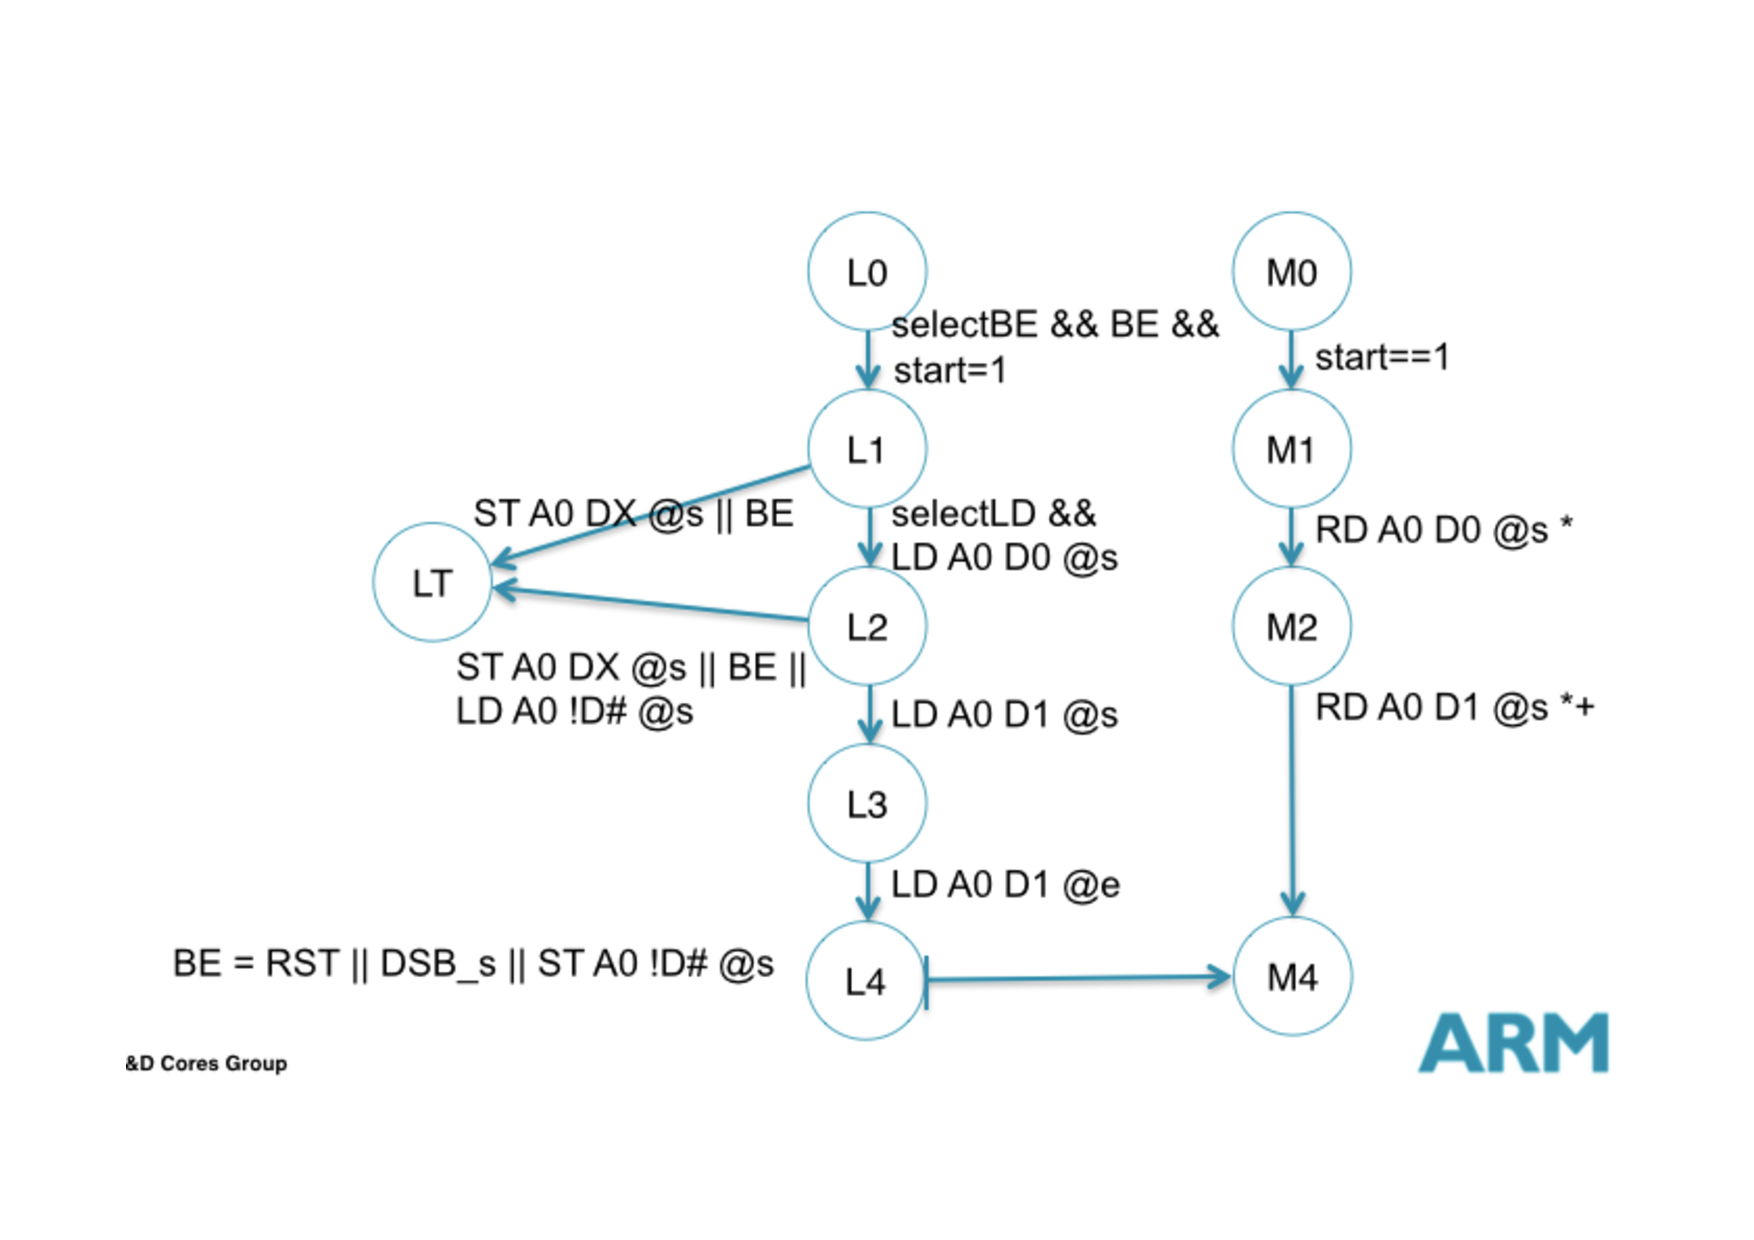
\includegraphics[width=.75\textwidth]{figures/loadload.pdf}
\caption{Load Load dog (source: difts14 talk)}
\label{fig:load-load-dog}
\end{figure}

\section{DOGs as First Order Logic Formulas}

A DOG implicitly structures events using different orders such as clock-time order and star order.
%
We can make this explicit by consider a first-order formula that represents the semantics of the DOG.

Give a DOG we consider the set of implications specified by the graph.
%
Each implication is transformed into a formula and the first-order formula of the whole DOG is the \emph{conjunction} of these formulas.

We assume that each implication is of the form $(S_1 \wedge S_2 \wedge \cdots) \mapsto (T_1 \vee T_2 \vee \cdots)$.
%
By substituting each state with an equivalent formula we transform the implication into a first-order implication.
%
We call each $S_i$ a \emph{triggering state} and each $T_i$ an \emph{accepting state}.
%
For each (triggering or accepting) state $U$ we consider all paths $P_0, P_1, \dots$ from the initial state of the FSM (containing $U$) to $U$.
%
Each path $P_i$ is transformed into a path-formula $f_i$ so that the formula for $U$ is the \emph{disjunction} of these path-formulas (i.e., $\bigvee f_i$).

In the following we assume the path is a sequence of states $U_0, \dots, U_{final}$.
%
Consider the expressions that transition the states of the path.
%
If the expression contains events then we first generate a fresh (event) variable that corresponds to these events.
%
This is the concrete event from a trace that matches an event of the expression, allowing the edge to transition.
%
For example, the expression \texttt{selectBE \&\& BE \&\& start = 1} between states \state{L0} and \state{L1} in Figure~\ref{fig:load-load-dog} uses the events $E = \{\textsf{reset}, \textsf{dsb@s}, \textsf{ST(A0,!D\#)@s}\}$.
%
This is denoted $(e \match E)$ and we call $e$ the match variable.
%
\subsection{Clock-time order}
%
For each pair of edges $U \xrightarrow{expr} U' \xrightarrow{expr'} U''$ in the path where $e$ and $e'$ are the corresponding match variables for the expressions $expr$ and $expr'$ we generate the following \emph{path constraint}:
%
\[
e \leq_{ct} e'
\]
%
For example, in Figure~\ref{fig:load-load-dog}, the path $\state{L0} \xrightarrow{expr_0} \state{L1} \xrightarrow{expr_1} \state{L2} \xrightarrow{expr_2} \state{L3} \xrightarrow{expr_3} \state{L4}$ yields the path constraint $e_0 \leq_{ct} e_1 \leq_{ct} e_2 \leq_{ct} e_3$ where $e_i$ is the corresponding match variable for $expr_i$.

\subsection{Vacuous escapes}
%
In Figure~\ref{fig:load-load-dog}, the transitions to state \state{LT} are \emph{vacuous escapes} because if any of these transitions is taken then the triggering state \state{L4} is unreachable.
%
We encode this as part of the \emph{path constraint} by generating a fresh match variable for each vacuous escape transition.
%
For example, if $x_0$ is the corresponding match variable for the vacuous escape transition $\state{L1} \rightarrow \state{LT}$ then we encode:
\[
\neg (\exists x_0 : e_0 \leq_{ct} x_0 \leq_{ct} e_1)
\]
%
and similarly, for the other escape transitions.

\subsection{Star order}
%
If the path contains a pair of expressions containing \emph{star} events then we generate constraints using Table~\ref{table:star} where $e$ (respectively $f$) is the match variable corresponding to the event expression \texttt{a} (respectively \texttt{b}).
%
Note that it is acceptable for clock-time and star-order to `contradict'.
%
For example, $f \leq_{ct} e \wedge e <_{so} f$.

\begin{table}[h]
\caption{Star ordering constraints}
\label{table:star}
\begin{tabular}{lll}
\toprule
\textbf{Event expression pair} & \textbf{Interpretation}   & \textbf{Formula} \\
\midrule
\texttt{a}, \texttt{b*+}       & pure alpha                & $e <_{so} f$ \\
\texttt{a}, \texttt{b*-}       & pure beta                 & $f <_{so} e$ \\
\texttt{a}, \texttt{b*!+}      & not alpha (beta or gamma) & $e =_{so} f \vee f <_{so} e$ \\
\texttt{a}, \texttt{b*!-}      & not beta (alpha or gamma) & $e =_{so} f \vee e <_{so} f$ \\
\bottomrule
\end{tabular}
\end{table}

\subsection{Complete events}
%
If a path contains a \texttt{COMPLETE} event then we must encode the following condition.
%
Let $e$ be the match variable corresponding to the complete event and $\mathsf{starts}$ be the set of match variables corresponding to the event expressions along the path up to the complete event.
%
Then $\mathsf{isComplete}(e, \mathsf{starts})$ is defined as
%
\begin{align*}
\exists x \in \mathsf{starts} & : e\; \mathsf{isEndFor}\; x \wedge \\
\forall s \in \mathsf{starts} & : \exists u \in Ev : u\; \mathsf{isEndFor}\; s \wedge u \leq_{ct} e \\
\end{align*}

\subsection{Syncs}

We now consider if the path is taken from the load-store or read-write domain.
%
\subsection{Load-Store Domain Path-Formulas}
%
\NCComment{Fresh variables, match structure, clock-time of path, vacuous escapes}

\subsection{Read-Write Domain Path-Formulas}
%
\NCComment{Filter preload path, Fresh variables, match structure, clock-time of path, star constraints, negated adjacent paths}

\subsection{Implementation}

An implementation of this transformation is given here: \url{https://github.com/nchong/dogir}.

\subsection{Daryl's alternative transformation}

\subsection{Alternative: Deep embedding in Coq/HOL}

\section{Hand-written \litmus{coRR} proof}
%
Using formula generated from load-load DOG we can reason about the \litmus{coRR} test.

\section{Hand-written \litmus{coRW1} proof}

\begin{verbatim}
  // [x] = 0 initially
  // P0
  LDR r0, [x]
  STR [x], #1
\end{verbatim}

The outcome $\texttt{r0} = 1$ is forbidden due to the \axiom{SC-PER-LOC} axiom.

\subsection{Load-Store DOG formula}

\begin{figure}[p]
\begin{verbatim}
exists sync :
  exists e0 e1 e2 e3 :
    (* match structure *)
    e0 match BE /\
    e1 match { LD(A0,D0)@s } /\
    e2 match { ST(A0,D1)@s } /\
    isComplete(e3, { e0, e1, e2 }) /\
    e0 = sync /\
    (* ct path constraint *)
    e0 <=ct e1 <=ct e2 <=ct e3 /\
    (* vacuous escapes *)
    not (exists x0 : x0 match { ST(A0,D1)@s } /\
                     x0 <=ct e0) /\
    not (exists x1 : x1 match { ST(A0,DX)@s } U BE /\
                     e0 <=ct x1 <=ct e1) /\
    not (exists x2 : x2 match { LD(A0,DX)@s, ST(A0,!D1)@s } U BE /\
                     e1 <=ct x2 <=ct e2)

  =>

  (* path ABD *)
  exists f0 :
    f0 match { RD(A0,D0)@s } /\
    sync <=ct f0 /\
    (* no step to bad state E *)
    not (exists y0 : y0 match { WR(A0,D1)@s } /\
                     f0 <=ct y0 /\
                     (f0 =so y0 \/ y0 <so f0))

  \/

  (* path ABCF *)
  exists f1 f2 :
    f1 match { WR(A0,D1)@s } /\
    f2 match { RD(A0,D0)@s } /\
    sync <=ct f1 <=ct f2 /\
    f2 <so f1
\end{verbatim}
\caption{Simplified formula for Uniproc Load-Store DOG}
\label{fig:loadstore-formula}
\end{figure}


\section{Related Work}

\bibliographystyle{alpha}
\bibliography{references}

\end{document}
